% !TeX encoding = UTF-8
% !TeX spellcheck = en_US
% !TeX root = ../../Thesis.tex

\chapter{Beam Characterization}
\label{ch:Beam Characterization}


\section{Aluminum foil}
\label{sec:Aluminum foil}

In \cref{fig:Front view of vacuum chamber (first iteration)} the inside of the 6-way cross of the first iteration is shown. On one side of the phosphor screen, aluminum foil was attached to simulate the aquadag coating inside a CRT. The beam was deflected on the aluminum foil and the BNC output was connected to ground through an ammeter to measure the beam current. As shown in \cref{fig:Difference in filament voltage and beam current between an open and sealed CRT} there is close to no difference in the filament voltage (and therefore heating power) between an opened and sealed CRT while the beam current on the aluminum foil varies widely. One possible reason could be that electrons scatter around and not all choose the wire path to ground. Therefore a Faraday cup (see \cref{sec:Faraday cup}) was used in the second iteration.
In \cref{fig:Front view of vacuum chamber (first iteration)} the inside of the 6-way cross of the first iteration is shown. On one side of the phosphor screen, aluminum foil was attached to simulate the aquadag coating inside the cut CRT. The beam was deflected on the aluminum foil and the BNC output was connected to ground through an ammeter to measure the beam current. As shown in \cref{fig:Difference in filament voltage and beam current between an open and sealed CRT} there is close to no difference in the filament voltage (and therefore heating power) between an opened and sealed CRT while the beam current on the aluminum foil varies widely. One possible reason could be that electrons scatter \correction{skip: around and not all choose the wire path to ground}. Therefore, a Faraday cup (see \cref{sec:Faraday cup}) was used in the second iteration.


\begin{figure}[h]
	\centering
	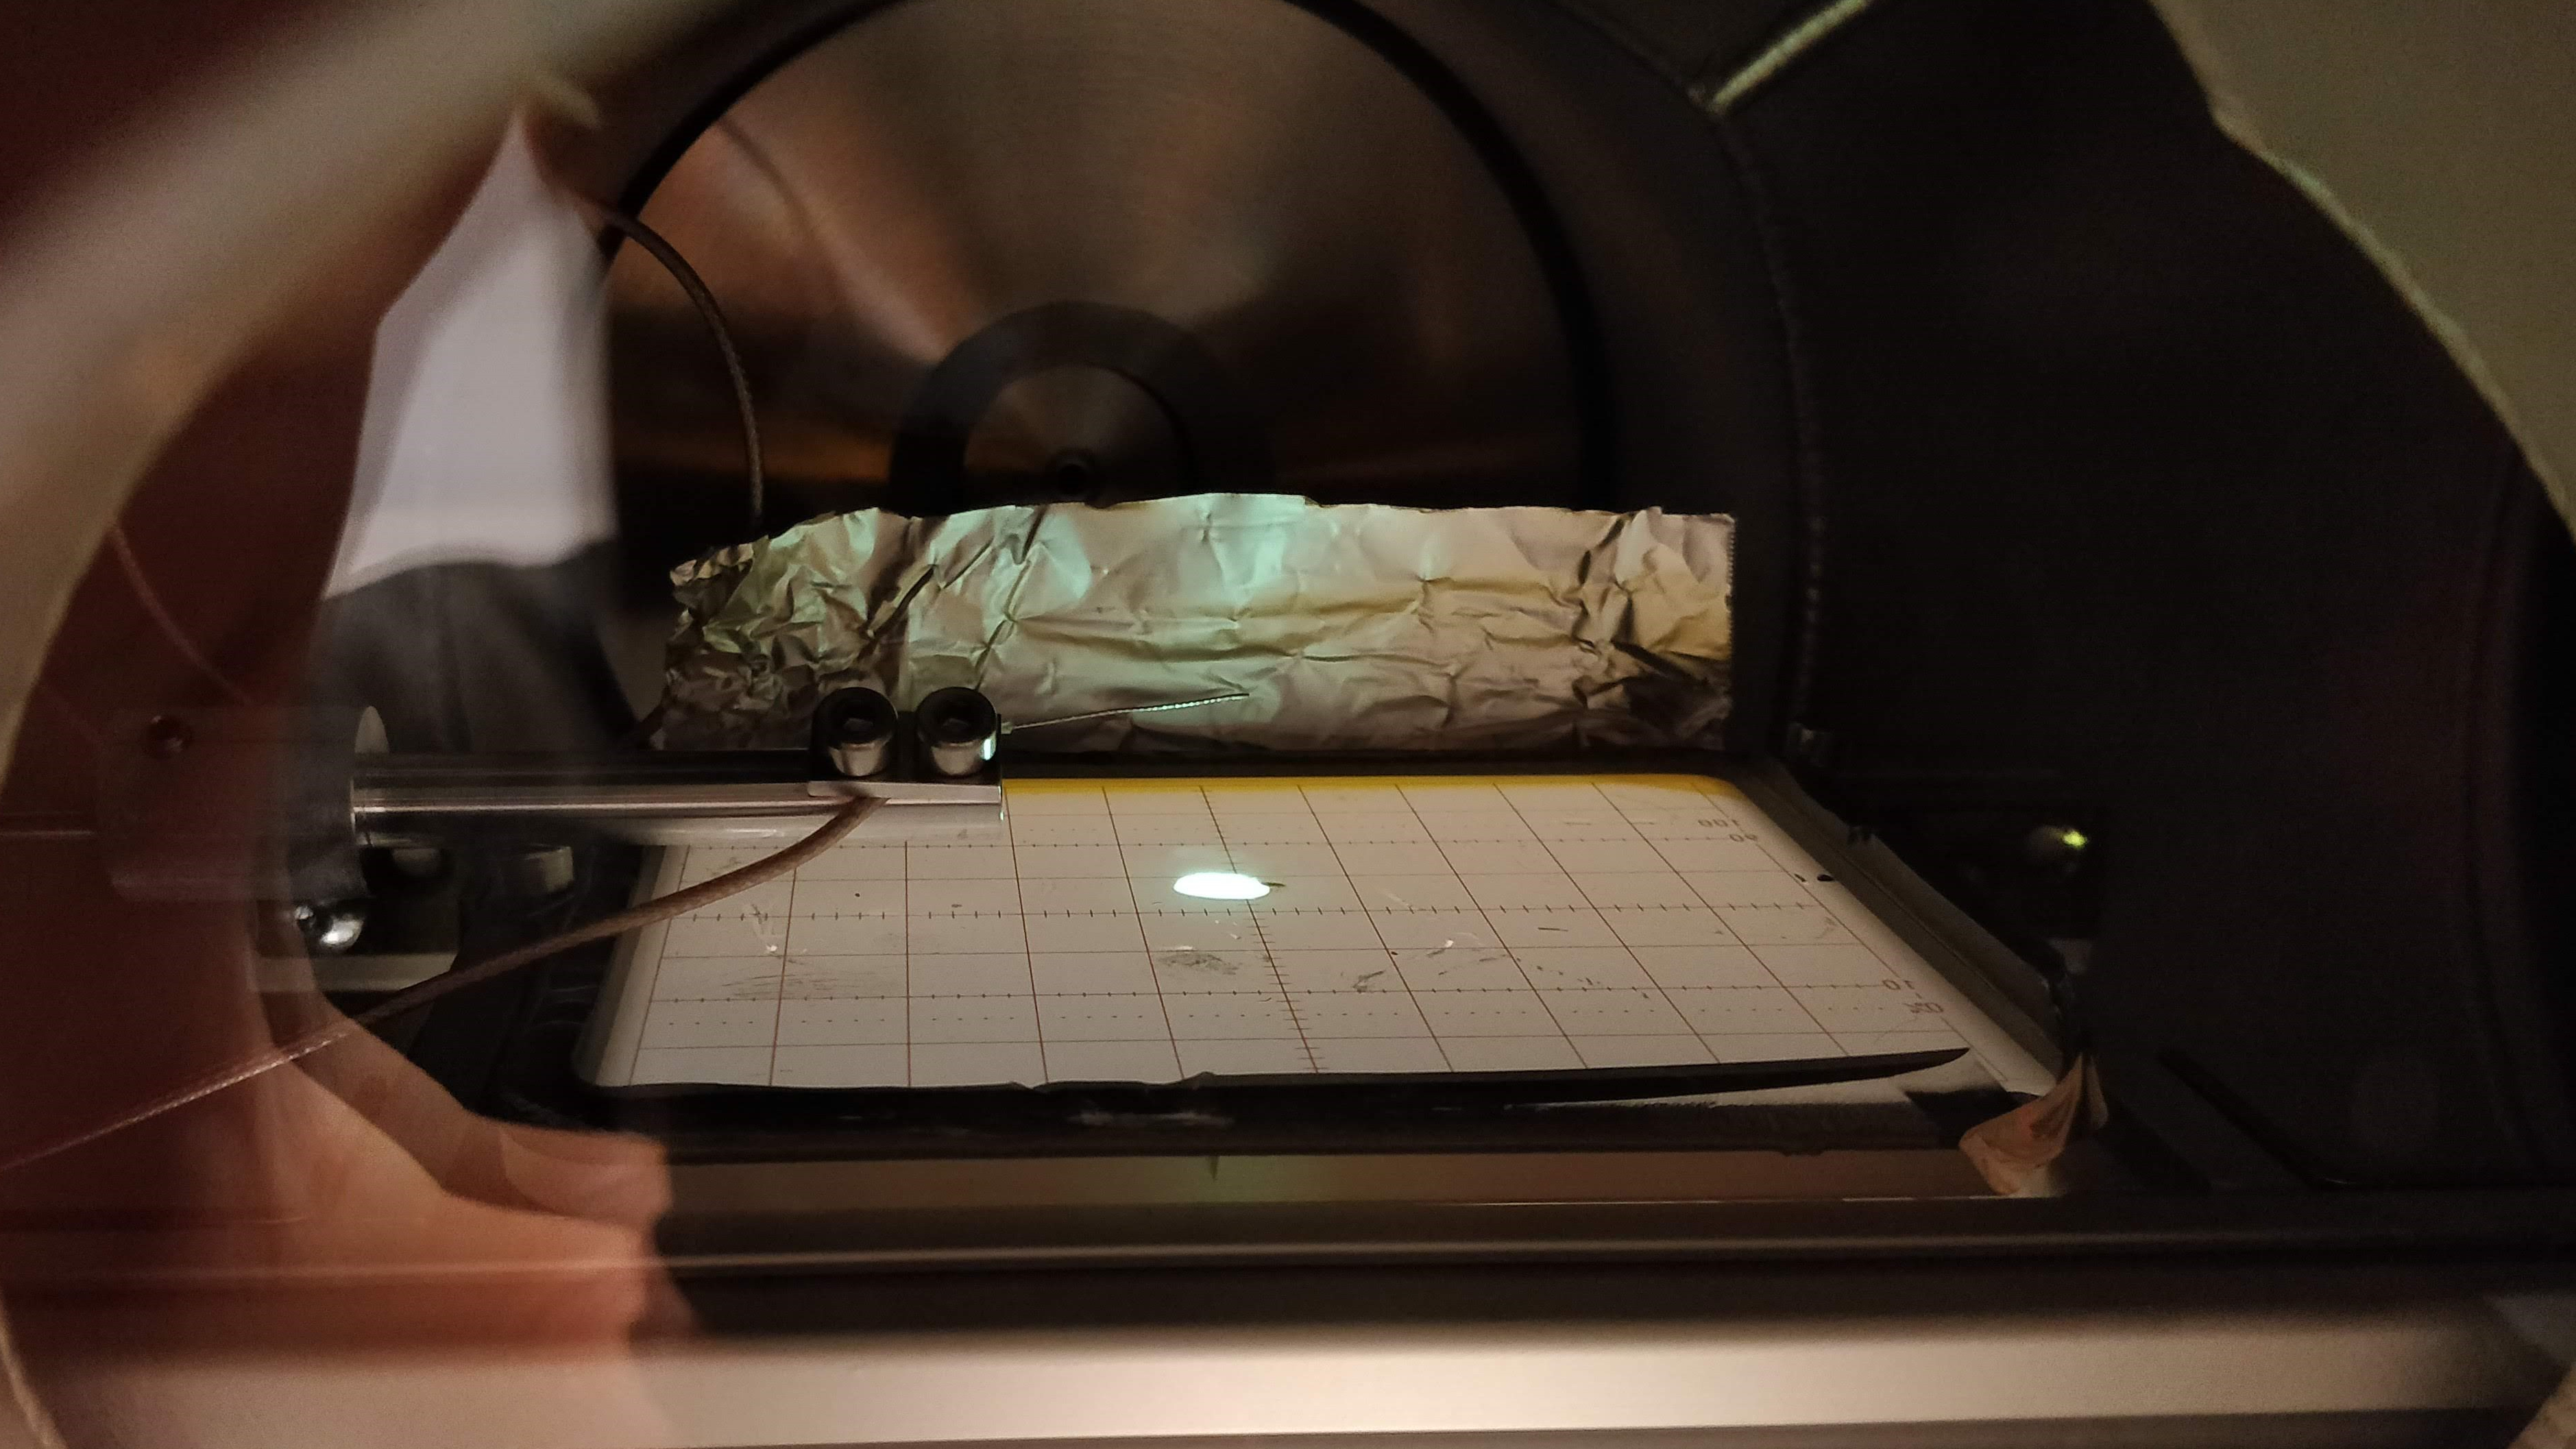
\includegraphics[width=0.9\textwidth]{./Chapters/beam-characterization/center_image}
	\caption{Front view of vacuum chamber (first iteration).}
	\label{fig:Front view of vacuum chamber (first iteration)}
\end{figure}


\begin{figure}[ht]
	\centering
	
	\begin{tikzpicture}
		% !TeX encoding = UTF-8
% !TeX spellcheck = en_US
% !TeX root = ../../Thesis.tex

\begin{groupplot}[
		group style={
			group size=2 by 1,
			horizontal sep=0.15\textwidth}, %0.1\textwidth},
		width=0.5\textwidth,
		height=0.5\textwidth]
	
	%1st plot
	\nextgroupplot[
		%title={},
		xlabel={filament current/\si{\milli\ampere}},
		ylabel={filament voltage/\si{\volt}},
	%	xmin=5, xmax=7.5,
	%	ymin=0, ymax=0.5,
		legend style={at={(0.05, 0.95)}, anchor={north west}},
		legend cell align={left}]
	
	\addplot+[
		black,
		only marks,
		mark=*,
		mark size=2pt,
		mark options={solid}]
	table [x=current_filament, y=voltage, col sep=comma]{./Chapters/beam-characterization/data_aluminum_foil_opened.csv};
	\addlegendentry{open}
	
	\addplot+[
		blue,
		only marks,
		mark=*,
		mark size=2pt,
		mark options={solid}]
	table [x=current_filament, y=voltage, col sep=comma]{./Chapters/beam-characterization/data_aluminum_foil_sealed.csv};
	\addlegendentry{sealed}
	

%	%2nd plot
	\nextgroupplot
	[
	%title={},
	xlabel={filament current/\si{\milli\ampere}},
	ylabel={beam current/\si{\micro\ampere}},
%	xmin=5, xmax=7.5,
	ymin=0, %ymax=0.5,
	legend style={at={(0.05, 0.95)}, anchor={north west}},
	legend cell align={left},
	]
	
	\addplot+[
		black,
		only marks,
		mark=*,
		mark size=2pt,
		mark options={solid}	]
	table [x=current_filament, y=current, col sep=comma]{./Chapters/beam-characterization/data_aluminum_foil_opened.csv};
	\addlegendentry{open}
	
	\addplot+[
		blue,
		only marks,
		mark=*,
		mark size=2pt,
		mark options={solid}]
	table [x=current_filament, y=current, col sep=comma]{./Chapters/beam-characterization/data_aluminum_foil_sealed.csv};
	\addlegendentry{sealed}
\end{groupplot}
	\end{tikzpicture}
	
	\caption{Difference in filament voltage and beam current between an open and sealed CRT.}
	\label{fig:Difference in filament voltage and beam current between an open and sealed CRT}
\end{figure}

\section{Faraday cup}
\label{sec:Faraday cup}


In order to accurately measure the beam current, a Faraday cup was built. A schematic is shown in \cref{fig:Schematics of Faraday cup}. A copper tube was cut at an \ang{45} angle on one side and a Cu-sheet was soldered at the top and bottom. A small hole of around \SI{5}{\milli\meter} was drilled at the top and a coaxial cable was attached on the mantle which connects to a BNC feedthrough at the top of the chamber. The small opening and bent floor were made in order to reduce backscattering as indicated by blue arrows. At the top surface a phosphor coating was applied in order to make the beam visible which made it easier to guide it into the opening hole.
In order to accurately measure the full beam current, a Faraday cup was built. A schematic is shown in \cref{fig:Schematics of Faraday cup}. A copper tube was cut at an \ang{45} angle on one side and a Cu-sheet was soldered at the top and bottom. A small hole of around \SI{5}{\milli\meter} was drilled at the top and a coaxial cable was attached on the mantle which connects to a BNC feed through at the top of the chamber. The small opening and angled floor were added, in order to reduce electron loss through back scattering, as indicated by blue arrows in \cref{fig:Schematics of Faraday cup}. At the top surface a phosphor coating was applied, in order to make the beam visible. This made it easier to guide it into the opening hole.


\begin{figure}[h]
	\centering
	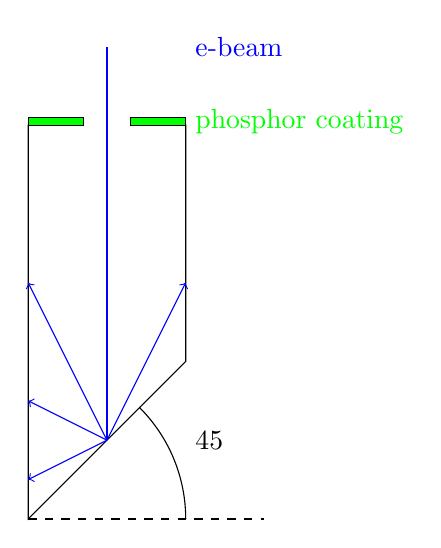
\begin{tikzpicture}
		% !TeX encoding = UTF-8
% !TeX spellcheck = en_US
% !TeX root = ../../Thesis.tex


%\draw [help lines] (-2, -2) grid (2, 5);


% cup
\draw (-0.3, 4) -- (-1, 4) -- (-1, -1) -- (1, 1) -- (1, 4) -- (0.3, 4);

% electron beam
\draw [blue] (0, 5) -- (0, 0);
\draw [blue, ->] (0, 0) -- (-1, -0.5);
\draw [blue, ->] (0, 0) -- (-1, 0.5);
\draw [blue, ->] (0, 0) -- (-1, 2);
\draw [blue, ->] (0, 0) -- (1, 2);
\node [right] at (1, 5) {\textcolor{blue}{e-beam}};

% 45 degree angle
\draw [dashed] (-1, -1) -- (2, -1);
\draw(-1+2, -1)arc [start angle=0,end angle=45, radius=2];
\node [right] at (1, 0) {\ang{45}};

% phosphor coating
\draw [fill=green] (-1, 4) rectangle (-0.3 , 4.1);
\draw [fill=green] (0.3, 4) rectangle (1, 4.1);
\node [right] at (1, 4.05) {\textcolor{green}{phosphor coating}};
	\end{tikzpicture}
	
	\caption{Schematics of Faraday cup.}
	\label{fig:Schematics of Faraday cup}
\end{figure}

With this improved setup, the beam current was measured again. A summary is shown in \cref{fig:Beam current dependence on heater current}. It can be seen that a current of over \SI{300}{\micro\ampere} was achieved, which is more than the necessary amount for the experiment. A problem is the fact, that the current is not stable. A measurement on the next day under the same settings resulted in a current between \SIrange{50}{120}{\micro\ampere}.
With this improved setup, the beam current was measured again (\cref{fig:Beam current dependence on heater current}). It can be seen, that a current of over \SI{300}{\micro\ampere} was achieved, which is more than the necessary amount for the experiment. However, through this measurement it became evident, that the current is not stable. A measurement on the next day under the same settings resulted in a current between \SIrange{50}{120}{\micro\ampere}.

\begin{figure}[h]
	\centering
	\begin{tikzpicture}
		% !TeX encoding = UTF-8
% !TeX spellcheck = en_US
% !TeX root = ../../Thesis.tex


	
%	%1st plot
%	\nextgroupplot[
%		%title={},
%		xlabel={filament current/\si{\milli\ampere}},
%		ylabel={filament voltage/\si{\volt}},
%	%	xmin=5, xmax=7.5,
%	%	ymin=0, ymax=0.5,
%		legend style={at={(0.05, 0.95)}, anchor={north west}},
%		legend cell align={left}]


\begin{axis}[
		%title={},
		xlabel={filament current/\si{\milli\ampere}},
		ylabel={beam current/\si{\micro\ampere}},
		%xmin=5, xmax=7.5,
		%ymin=0, ymax=0.5,
		%legend style={at={(0.05, 0.95)}, anchor={north west}},
		%legend cell align={left}]
	]
	\addplot[
		black,
		only marks,
		mark=*,
		mark size=2pt,
		mark options={solid},
	]
	table [x=current_filament, y=current_beam, col sep=comma]{./Chapters/beam-characterization/data_Faraday_cup.csv};
\end{axis}
	\end{tikzpicture}

	\caption{Beam current dependence on heater current.}
	\label{fig:Beam current dependence on heater current}
\end{figure}

\section{Deflection frequency}
\label{sec:Deflection frequency}

This section describes a few observations that were made when letting the electron beam interact with a short piece of wire, that is mounted to the wobble stick. Originally, we hoped to be able to measure the beam waist, using the knives edge method, i.e. observing the current transported by the beam, while slowly moving a razor blade into the beam path. However the beam is bent, when it passes closely to a conductive part. Whenever we moved our wire close to the beam, the visible spot on the Phosphorous screen below was distorted. This will probably complicate the measurement of the beam waist in the future. 
This section describes a few observations, that were made when letting the electron beam interact with a short piece of wire, that is mounted to the wobble stick. Originally, we hoped to be able to measure the beam waist, using the knife edge method, i.e. observing the current transported by the beam, while slowly moving a razor blade through the beam path. However the beam is bent, when it passes closely to a conductive part. Whenever, we moved our wire close to the beam, the visible spot on the Phosphorous screen below was distorted. This will probably complicate the measurement of the beam waist in the future. 
When the wire is connected to an oscilloscope, one can see a sharp increase in voltage, when it is moved into the beam. This can be used to see whether our deflection plates work properly and to test how fast we are able to deflect the beam. If the beam oscillates back and forth on a straight line and crosses the wire on the midway point, we should see a spike in voltage on the wire, which repeats with twice the frequency of the beam. If the wire is not on the midway point, the periods between consecutive spikes should sum up to the period of the beam's oscillation (see \cref{fig:spikes}). At low frequencies we have indeed observed this behavior. As the frequency is increased, the magnitude of the signal decreases. This is easily explained by the fact that the remain time close to the wire is inversely proportional to the frequency and the amplitude of beams deflection. It was possible to see the spikes up to a frequency of \SI{100}{\kilo\hertz}, before they where obscured by noise and some other periodical, but so far unexplained artifacts.
At high deflection frequencies, the wire may also pick up some signal form the capacitive charging and discharging of the deflection plates and the corresponding oscillating electromagnetic field.
In order to be able to see what happens at higher frequencies, a higher beam current and a smaller deflection amplitude would be beneficial, however the most important factor in order to understand what is happening is better focus and a better beam shape.
In order to be able to see what happens at higher frequencies, a higher beam current and a smaller deflection amplitude would be beneficial. However, the most important factor in order to understand what is happening, is a better focus and a better beam shape.

% TODO: \usepackage{graphicx} required
\begin{figure}
	\centering
	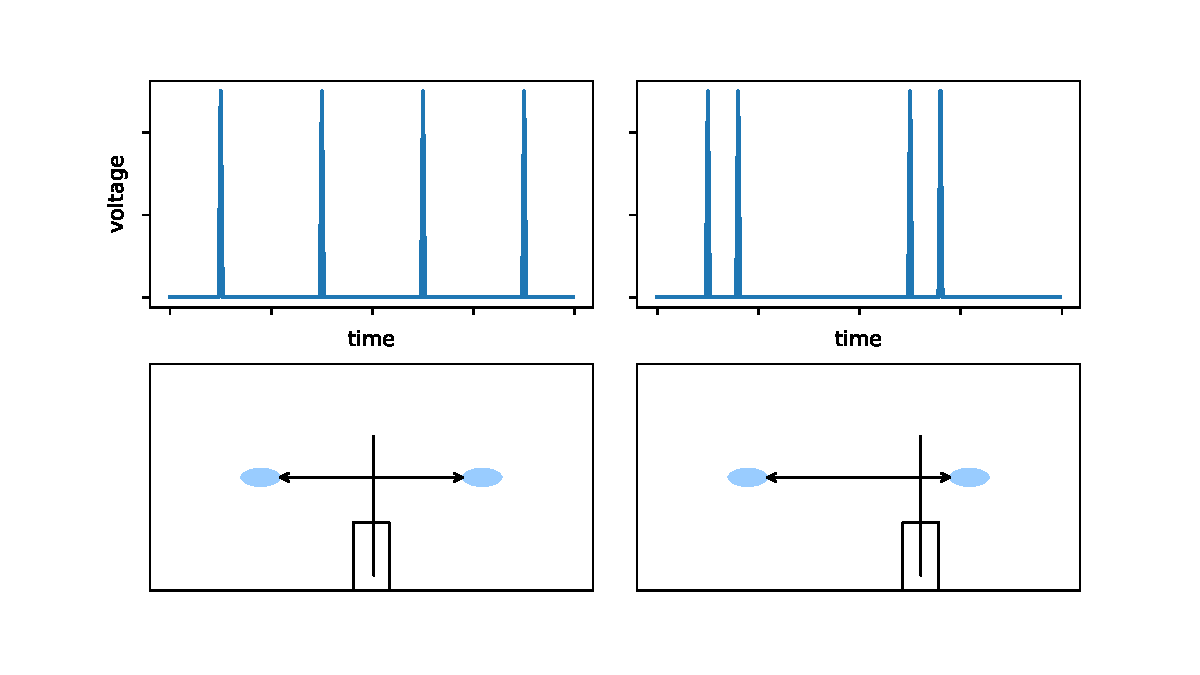
\includegraphics[width=0.8\linewidth]{Chapters/beam-characterization/Spikes}
	\caption{}
	\label{fig:spikes}
\end{figure}
\correction{caption missing}